\documentclass{beamer}
\beamertemplatenavigationsymbolsempty
\usepackage{tikz}
\usepackage{pgfplots}
\pgfplotsset{compat=1.18}
\begin{document}
\begin{frame}
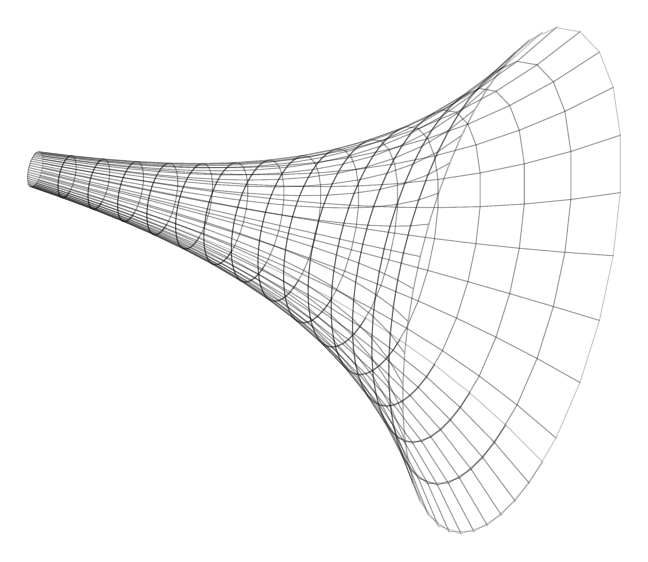
\begin{tikzpicture}[scale=1]
\begin{axis}[
hide axis,
view={25}{30},
scale=3,
unit vector ratio=2 1 1,
]
\addplot3[
mesh,
color=black,
opacity=0.2,
samples=40,
%restrict z to domain=-4:4,
restrict x to domain=-2:2,
]({x},{(2^x)*cos(deg(y))},{(2^x)*sin(deg(y))});
\end{axis}
\end{tikzpicture}
\end{frame}
\end{document}